\section{Applications}

\subsection{2D Lithophane}
A user sets the minimum thickness  $n$ and maximum thickness $m$.
Based on the material parameter transmittance $t$ as percentage of light after 1mm (more) thickness,
we calculate the thickness $h$ at each location based on the luminance $I$ there:
\begin{align}
p &= \frac{1}{\log_2 t}
\\
b &= 2^{(m-n)/p}
\\
h &= n + p \log_2 ( b + (1-b) I )
\end{align}


\begin{figure}[H]
\centering
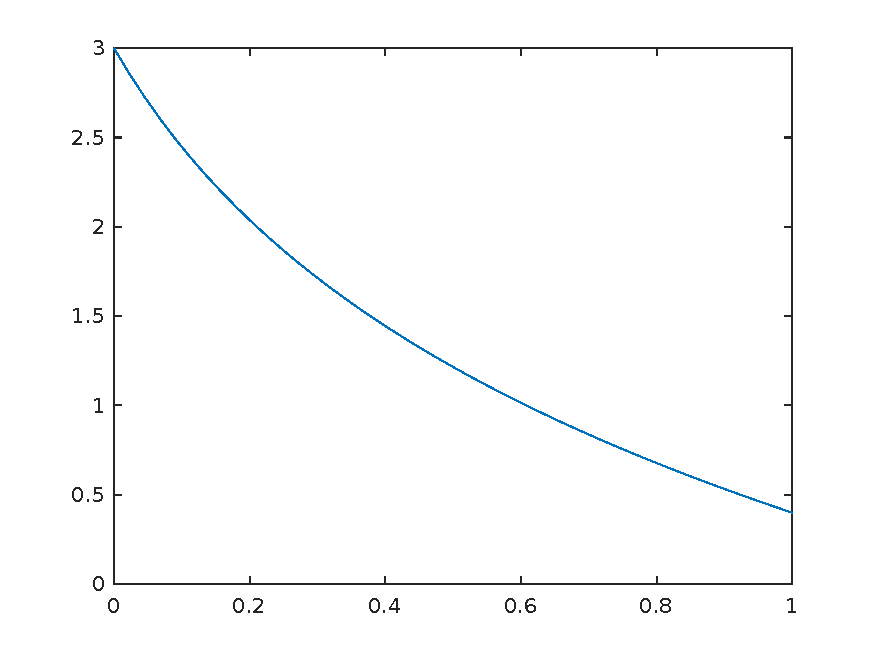
\includegraphics[width=.75\columnwidth]{sources/litho/luminance_to_thickness.pdf}
\caption{Mapping luminance to height for 2D lithophanes.}
\label{luminance_to_thickness}
\end{figure}






\subsection{3D Lithophane}
``The illuminance $E_\text{p}$ lux at a location $d$ metres from a point source of intensity $I$ candela is given by the cosine law of illumination,
$E_\text{p} = I \cos \theta / d^2$.''\cite{snow2001plant}
We relate the distances to the model: $E_\text{p} = I \cos \theta / (d_\text{rel} \cdot d_\text{max})^2 = d_\text{max}^2 I \cos \theta / d_\text{rel}^2$.
The scaling factor $d_\text{max}^2 I$ depends on the light source (intensity and location) and the 3D model.


The RGB values are scaled in order to prevent too dark requests which would correspond to too thick shell: $R' = E_\text{min} +  (1 - E_\text{min}) R$.
Likewise for G and B.

We assume a simple translucency model where twice the thickness implies squaring the fraction of transmitted light.
Suppose a thickness of $w=1$ corresponds to \SI{30}{\percent} absorbtion, so the transmittance is $\tau_1 = 0.7$.
Then a thickness of $w=2$ should correspond to a transmittance of $\tau = \tau_1^2 = 0.7^2 = .49$.
% A thickness of $w=4$ then corresponds to $\tau = (\tau_1^2)^2$.
In general $\tau = \tau_1^w$, so we derive that $w = \log_{\tau_1} \tau = \frac{\log \tau}{\log \tau_1} = c \log \tau$,
where $c$ and $\tau_1$ depend on the material.
The thickness of the shell at any location is determined by $w = c \log \frac{E_\text{p}}{E_\text{r}}$.

The requested luminance is computed from the texture image as $E_\text{r} = I_\text{r} \left( 0.212655 R^\gamma + 0.715158 G^\gamma + 0.072187 B ^\gamma \right)$, where $\gamma = 2.2$.
This formula comes from the official conversion from sRGB to CIE XYZ and taking the Y for luminance.
Zero light requires infinite thickness, so we introduce an $E_\text{min}$.
We might choose to cap all $E_\text{r}$ to lie above $E_\text{min}$, but that means we'd lose a range of brightnesses.
We instead choose to resize the range of requested brightnesses to be between min luminance and $1.0$.

$E_\text{p}$ depends on an unknown scaling factor $I$, and $E_\text{r}$ can be scaled at will.
The total ratio $\frac{E_\text{p}}{E_\text{r}}$ can therefore be scaled by some factor $b$:
$w = c \log b \frac{E_\text{p}}{E_\text{r}} = cb + c \log \frac{E_\text{p}}{E_\text{r}} = x + c \log \frac{E_\text{p}}{E_\text{r}}$
(Beware this formula can give negative values for $w$.)

We can choose $x$ so as to optimize the range of achievable brightnesses given the minimum and maximum thickness of the shell.
Finally, the offset is clamped to within the range $[0.4, 3.0]$ so that it is always manufacturable with a nozzle size of \SI{0.4}{\milli\meter} and is not too large.

For materials where $\tau_1 \to 1$ (i.e. $c \to 0$) the translucency is too high and the luminance modulation would require thicknesses which are too large.
For materials where $\tau_1 \to 0$ (i.e. $c \to -\infty)$ the translucency is too low and the luminance is modulated by a too small range in thicknesses.
The optimal $\tau_1$ depends on the size and geometry of the model as well as the texture colors.
See \url{https://www.photonics.com/Articles/Accurate_Transmission_Measurements_of_Translucent/a32297} on measurement of transmittance.
Also see \url{https://www.plasticsnet.com/doc/article-how-to-measure-translucent-materials-0001}


\hl{The ambient illuminance can be better approximated using existing algorithms.
We can render the object lit from within and bake the illumination into a separate texture channel.
That channel can then serve as input to our program.}


Performing offsets can sometimes produce self-intersections.
We therefore export the outer and inner shell and perform a boolean difference operation using existing tools (Blender).



\subsection{Variable thickness microstructures}
show the effect of the planned toolpath on the performance of varying thickness microstructures

Implement varying width for infill patterns in Cura?
